% 二段組にして日本語を使う
\documentclass[twocolumn]{jarticle}
\usepackage[top=30truemm,bottom=25truemm,left=20truemm,right=20truemm]{geometry}
% 画像を挿入するためのパッケージ
\usepackage[dvipdfmx]{graphicx,color}

% 著者を書くためのパッケージ
\usepackage{authblk}
% ハイパーリンクのためのパッケージ
\usepackage[dvipdfmx]{hyperref}
% ソースコード表現するためのパッケージ
\usepackage{listings}

% ソースコード内で日本語を入れるためのパッケージ, インストールが面倒だったらコメントアウトすればコンパイルできます。
\usepackage{jlisting}

% 数式を整えるためのパッケージ
\usepackage{amsmath}

% ソースコードに色を付ける
\lstset{
backgroundcolor={\color[gray]{.98}},
basicstyle={\small},
identifierstyle={\small},
commentstyle={\small\ttfamily \color[rgb]{0,0.5,0}},
keywordstyle={\small\bfseries \color[rgb]{0,0,0.8}},
ndkeywordstyle={\small},
stringstyle={\small\ttfamily \color[rgb]{0,0,1}},
frame={tb},
breaklines=true,
columns=[l]{fullflexible},
% numbers=left,
xrightmargin=0zw,
% xleftmargin=3zw,
numberstyle={\scriptsize},
stepnumber=1,
numbersep=1zw,
morecomment=[l]{//}
}
\title{\large\gt\LaTeX のインストールと使い方}

\author{\normalsize 長島康生}

\affil{\normalsize 慶應義塾大学環境情報学部4年 脇田研究会}

\date{2022/6/22}

\begin{document}
\maketitle
\section{はじめに}
\subsection{この文書について}
この文書では、TeX Liveのインストール方法と、VSCodeにおける環境構築について解説します。
この文書を読んでも、
\begin{itemize}
    \item VSCodeのインストール方法、使い方
    \item VSCode以外のエディターを利用した\LaTeX の使い方
    \item scheme-small以外のTeX Liveのインストール方法(後述します。)
    \item コマンドなどの具体的な解説。
\end{itemize}
などはわからないので各自調べてください。
\subsection{TeX Liveとは}
TeX Liveとは\cite[TeX Wiki]{TexLive} によると
\begin{quotation}
    TeX Live は TeX のディストリビューションです. TeX の超巨大な集大成ともいえるもので,現在では国際的に最も普及している最新の TeX ディストリビューションです.
\end{quotation}
で、TeX Liveには、\LaTeX を利用するために必要な機能や、パッケージマネージャーであるtlmgr など同梱されています。
また、Macには、Macに最適化されたTeX LiveであるMacTexが存在するため、Macの場合はこちらを使うのがいいでしょう

また、最初にTeX Liveの全機能(scheme-full)をインストールしようとすると、容量が大きいため、とても時間がかかります。そのため、必要最低限の機能をインストールするscheme-small(MacならBasicTex)でインストールするのを推奨します。そのため、この文書ではscheme-smallでインストールした場合について解説します。

\section{TeX Liveのインストール}
\subsection{linuxの場合}
\href{https://www.tug.org/texlive/acquire-netinstall.html}{Project GutenbergInstalling TeX Live over the Internet}から、install-tl-unx.tar.gz をダウンロードし、解凍、ディレクトリを移動して、
\begin{lstlisting}[language=bash]
$ sudo ./install-tl -scheme=small
\end{lstlisting}
インストールオプションがたくさん出てくる。デフォルトで良ければ、i を入力してインストールします。インストールが終了したら、PATH, MANPATH, INFOPATHが表示されるので環境変数に追加するのを忘れないでください。

\subsection{Macの場合 \cite{BasicTeX} }

\subsubsection{brewを使う}
\begin{lstlisting}[language=bash]
$ brew install --cask basictex
\end{lstlisting}

\subsubsection{brewを使わない}
\href{https://tug.org/mactex/morepackages.html}{MacTex Smaller Download}からBasicTex.pkgをダウンロードし、ダウンロードしたファイルをダブルクリック

\section{tlmgrで日本語対応}
tlmgrというTexLiveのパッケージマネージャーを使います。
まず、tlmgrを最新版にアップデートします。
\begin{lstlisting}
$ sudo tlmgr update --self --all
\end{lstlisting}
そして日本語対応のためのパッケージをインストールします。
\begin{lstlisting}
$ sudo tlmgr install \
    collection-basic \
    collection-latex \
    collection-latexrecommended \
    collection-latexextra \
    collection-fontsrecommended \
    collection-langjapanese
\end{lstlisting}
これで TeX Liveで日本語が使えるようになったはずです。

\section{VSCodeの設定}
まず、任意の場所にディレクトリを作成し、VSCodeで開きます。

そして、拡張機能から\ref{vscode} LaTeX Workshopをインストールします。
\begin{figure}[h]
    \centering
    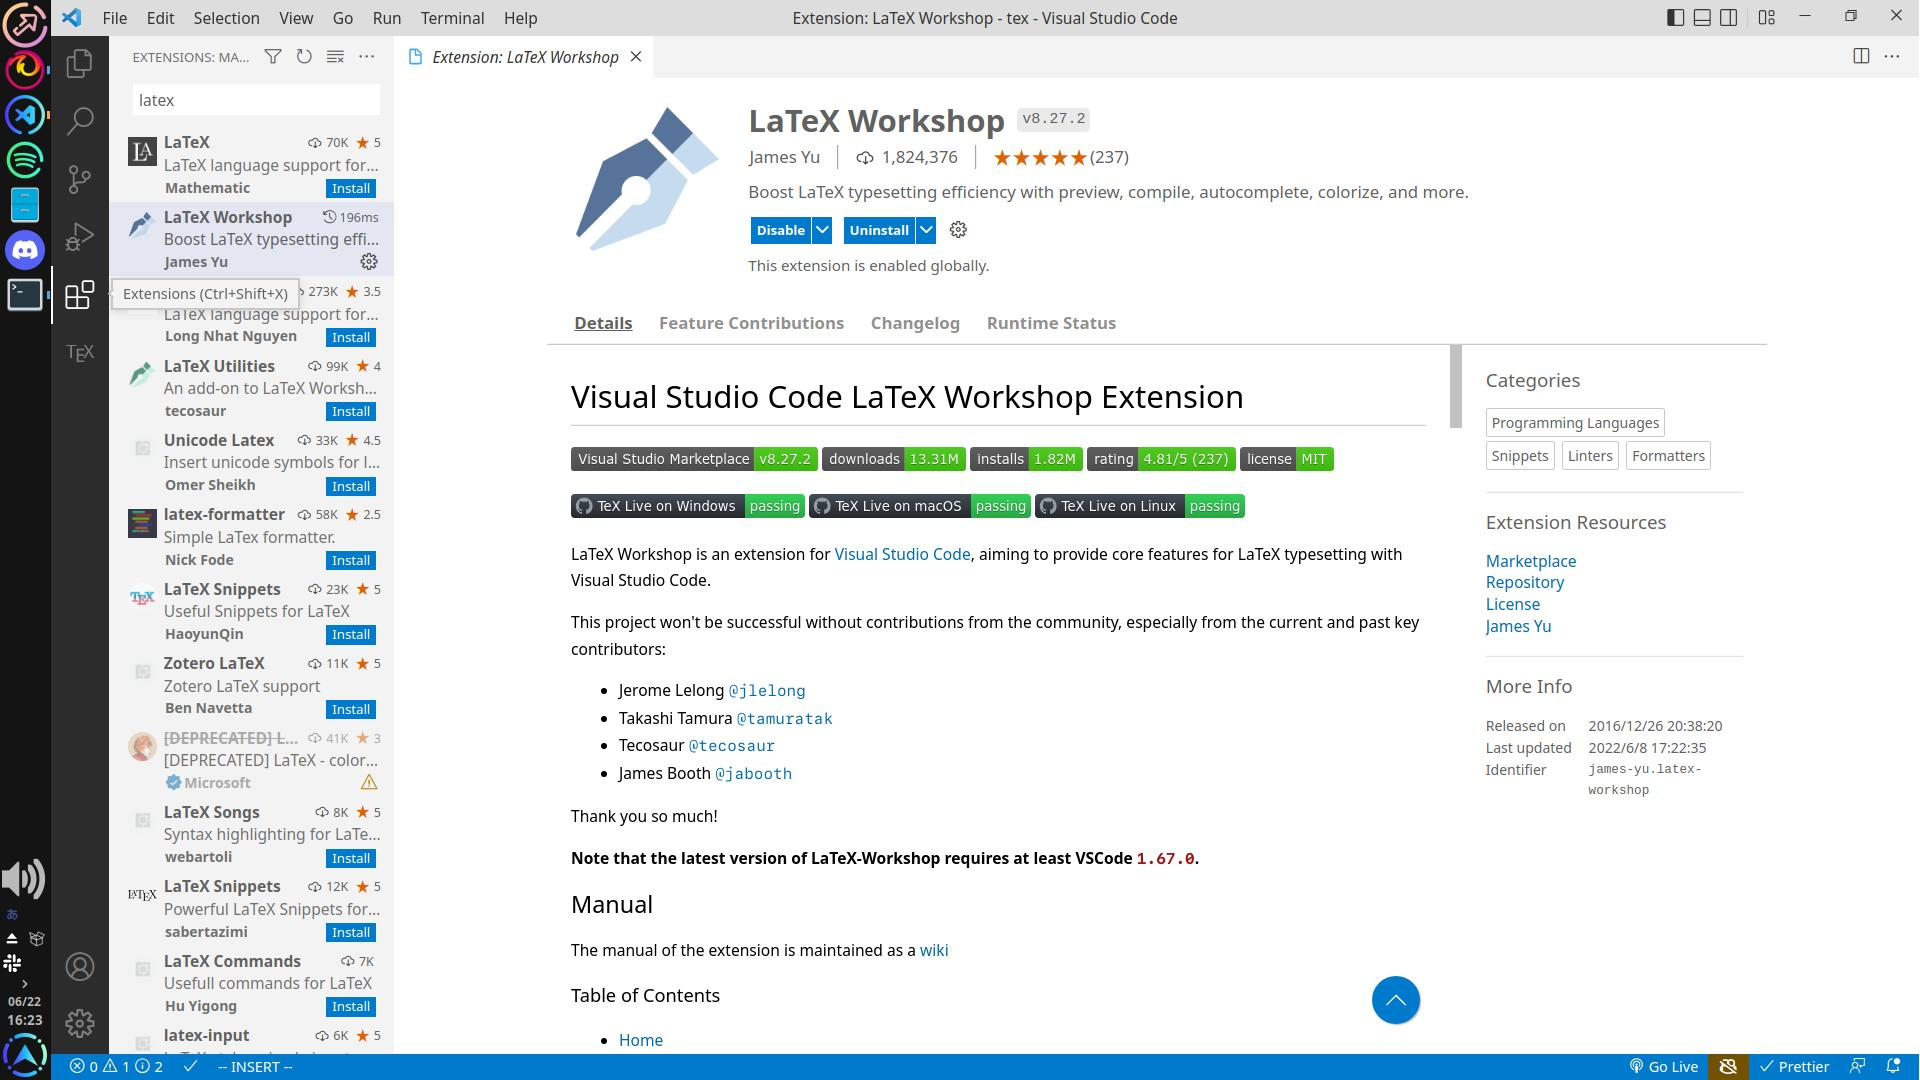
\includegraphics[keepaspectratio, scale=0.1]{vscode.jpg}
    \caption{LaTex Workshop}
    \label{vscode}
\end{figure}

.vscode/setting.jsonというファイル(なかったら作成)に\ref{setting}を書いてください。
これは、複数のコマンドを一括で実行できるようにするための設定です。
この設定によって、LaTeX Workshopのサイドバーにレシピが追加されます。
latex-workshop.latex.recipe.defaultを変更することで、ファイルを保存したときに実行されるコマンドを変更することができます。

\section{実際に書いてみる}
新しくsample.texというファイルを作り、次のように書いてください。
\lstinputlisting[caption=sample.tex, language=TeX]{sample.tex}

そして、ファイルを保存、もしくはTeX Workshopのサイドバー $\to$ Build LaTeX project $\to$ Recipe: convert pdfをクリックすることで、PDFが生成されます。
Ctl+Alt+V を押すことでVSCode内で見ることもできます。
\ref{run-recipe}のようになっていれば成功です。
\begin{figure}[b]
    \centering
    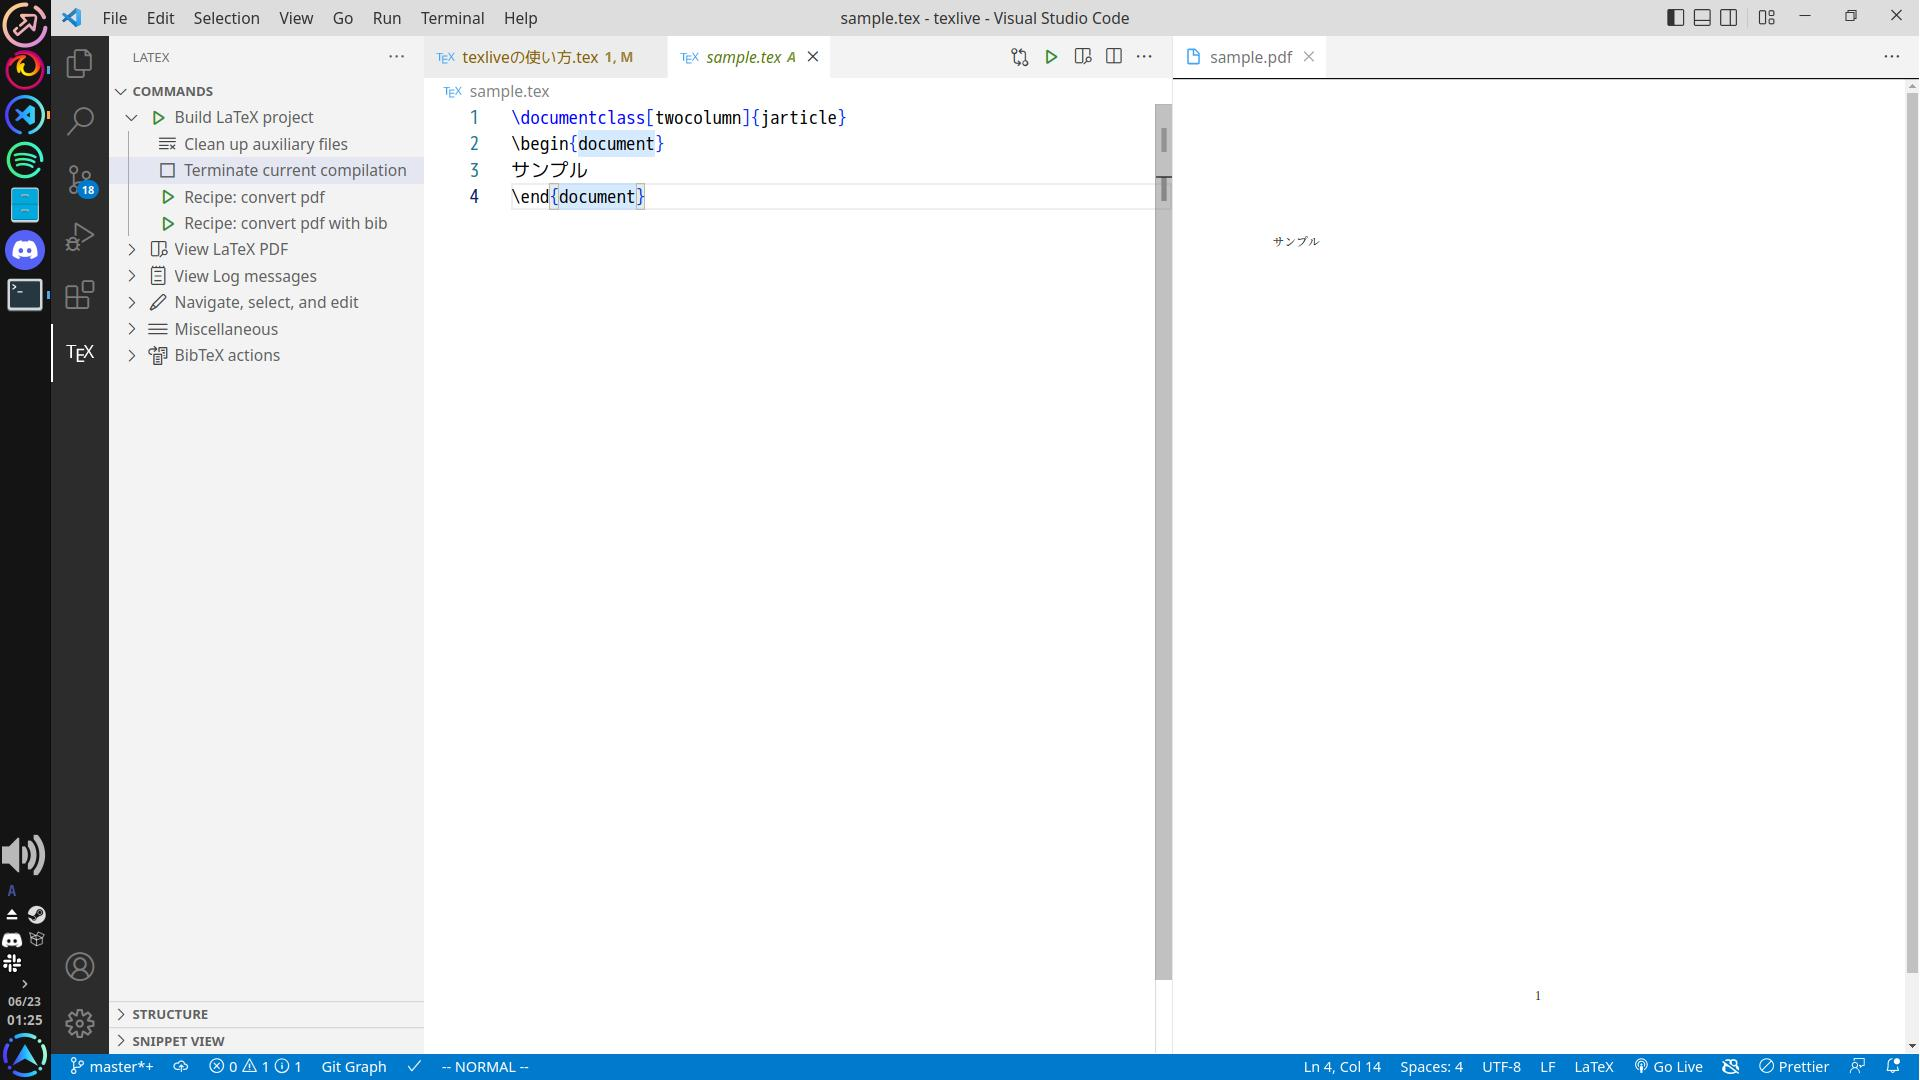
\includegraphics[keepaspectratio, scale=0.1]{run-recipe.jpg}
    \caption{レシピを実行したときの画面}
    \label{run-recipe}
\end{figure}

\section{参考文献を入れる}
参考文献にはbibtex(日本語環境ではpbibtex)を使います。
論文が掲載されているサイトからbibtex形式で取得できることが多いので、それを使うと便利です。
sample-bib.texとsample.bibを新しく作り、以下のように書いてください
\lstinputlisting[caption=sample-bib.tex,language=TeX]{sample-bib.tex}
\lstinputlisting[caption=sample.bib]{sample.bib}
そして、今度はRecipe: convert pdf with bib をクリックし、Ctl+Alt+V を押してください
\ref{run-recipe-with-bib}のようになっていれば成功です。
\begin{figure}[b]
    \centering
    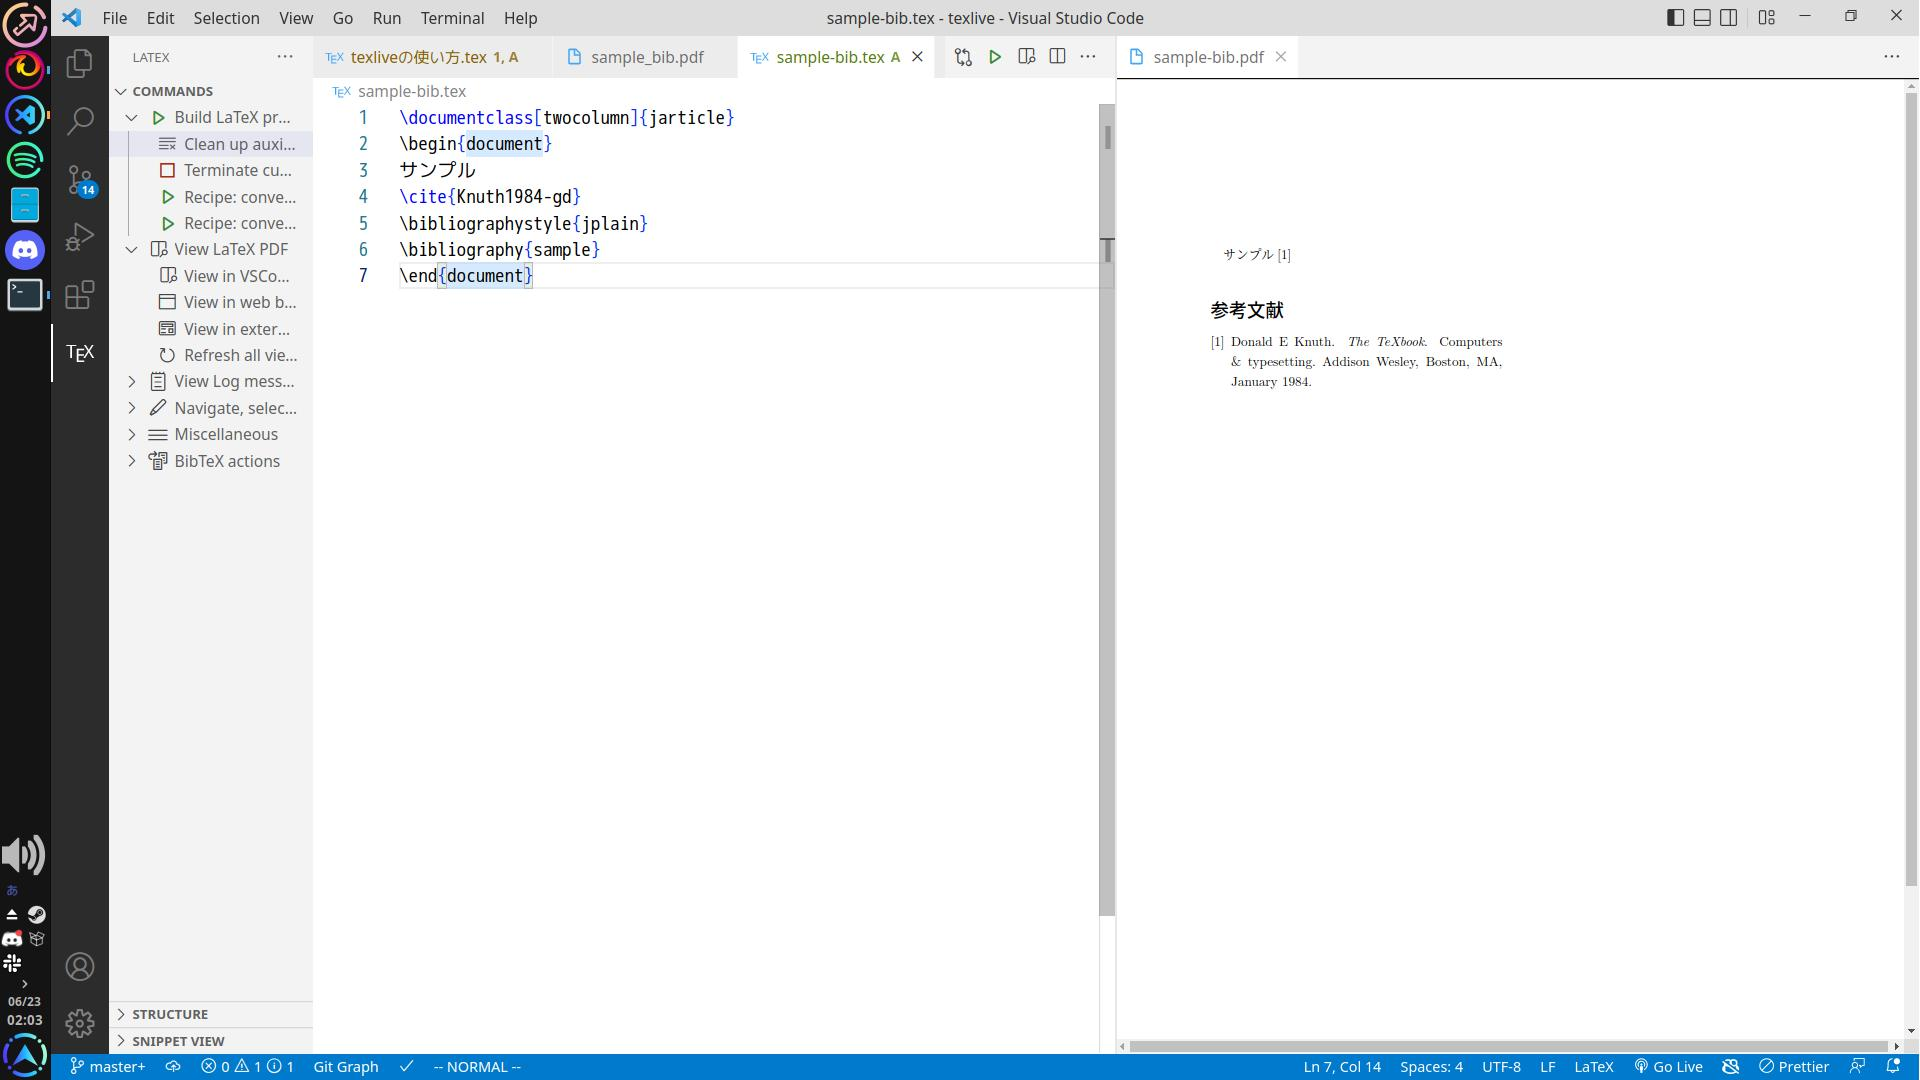
\includegraphics[keepaspectratio, scale=0.1]{run-recipe-with-bib.jpg}
    \caption{参考文献付きレシピを実行したときの画面}
    \label{run-recipe-with-bib}
\end{figure}

\section{数式の書き方}
あくまで例示で、様々な書き方があるので各自調べてほしいです。
これが、
\begin{lstlisting}
\begin{align*}
    \frac{\partial \mathbf{u}}{\partial t} & = - (\mathbf{u} \cdot \nabla)\mathbf{u} + v \nabla ^2 \mathbf{u}+f, \\
    \frac{\partial \rho}{\partial t}       & = -(\mathbf{u} \cdot \nabla) \rho + k\nabla^2 \rho + S
\end{align*}
\end{lstlisting}
こうなります。
\begin{align*}
    \frac{\partial \mathbf{u}}{\partial t} & = - (\mathbf{u} \cdot \nabla)\mathbf{u} + v \nabla ^2 \mathbf{u}+f, \\
    \frac{\partial \rho}{\partial t}       & = -(\mathbf{u} \cdot \nabla) \rho + k\nabla^2 \rho + S
\end{align*}
文章中にも数式$(\mathbf{u} \cdot \nabla)\mathbf{u}$を書けます。
\begin{lstlisting}
文章中にも数式$(\mathbf{u} \cdot \nabla)\mathbf{u}$を書けます。
\end{lstlisting}

\section{その他}
章の書き方や画像の挿入の仕方などはこの文書のソースコードを読んだり、Webで調べて書いてください。
この文書を作成する際に、ソースコード内に日本語を表示するため、jlistingパッケージを別途インストールしてコンパイルしています。
\cite[この記事]{jlisting}を参考にインストールするか、
\begin{lstlisting}
\usepackage{jlisting}
\end{lstlisting}
をコメントアウトすればコンパイルできます。

\begin{figure*}[t]
    \lstinputlisting[caption=setting.json]{.vscode/settings.json}
    \label{setting}
\end{figure*}
\bibliographystyle{jplain}
\bibliography{references}

\end{document}